%\documentclass[handout]{beamer}
\documentclass{beamer}

\usepackage[english]{babel}
\usepackage[latin1]{inputenc}
\usepackage{textpos}
\usepackage{epstopdf}
\epstopdfsetup{update}
%\usepackage{pgfpages}
%\pgfpagesuselayout{resize to}[letterpaper,landscape]
%\usepackage{epstopdf}
%\epstopdfsetup{update}
\usepackage{pgfplots}
\usepackage{pgfbaseimage}
\usepackage{amsmath} 						%More mathematical
\usepackage{multirow}
%\usepackage[absolute,overlay]{textpos}
%\usepackage[tikz]{bclogo}
%\usepackage{etoolbox}
% listings for matlab code:
\usepackage{listings}
%\usepackage[autolinebreaks, useliterate]{mcode}
\lstset{backgroundcolor=\color[gray]{0.9}}

\usepackage{chemplants}
\usepackage{cancel}
\usepackage{graphicx}
\usetikzlibrary{math}
\usepackage{wasysym}
\usepackage{marvosym}

\usetikzlibrary{shapes.arrows}
\tikzset{My Arrow Style/.style={single arrow, draw=green!40!gray, very thick, fill=green!20!gray!10, anchor=base, align=center,text width=2cm,text=green!40!gray,rotate=-90,minimum width=0.5cm, inner sep=1mm, minimum height=0.5cm}}
\newcommand{\MyArrow}[2][]{\tikz[baseline] \node [My Arrow Style,#1] {#2};}

%-------------------------------------------------
% FOOTER
%
% Choose your footer style, by commenting other options:
%
%% - Clean: no footer, except of page number
\mode<presentation>{\usetheme{presentationTemplateBiomathFClean}}
%%  - Info: a fixed footer with basic presenter information
%\mode<presentation>{\usetheme{presentationTemplateBiomathFInfo}}
%%  - Section: Provide the sections and current section in the footer 
%\mode<presentation>{\usetheme{presentationTemplateBiomathFSection}}
%-------------------------------------------------


%voor de hand-outs
%\usepackage{pgfpages}
%\pgfpagesuselayout{2 on 1}[a4paper,border shrink=5mm]

\title{\LARGE Modelling and Simulation \normalsize of Biosystems}
\title{Modelling and Simulation of Biosystems}
\author[Daniel Illana]{Daniel Illana Gonz\'alez} %(daniel.illanagonzalez@ugent.be)}
\subtitle{Practicum 1: Modelling with ODEs}
\date{Academic year 2024-2025}


\newcommand{\mtx}[2]
  {\left[\begin{array}{#1}#2\end{array}\right]}
\newcommand{\eqset}[1]
  {\left\{\begin{array}{rcl}#1\end{array}\right.}
\newcommand{\rbar}[2]
  {\left.#1\right|_{#2}}
\newcommand{\atwp}[1]
  {\rbar{#1}{\overline{X},\overline{U}}}

\usepackage{mdframed}

\newenvironment{opgave}[2][]{%
	\mdfsetup{%
		frametitle={%
			\tikz[baseline=(current bounding box.east),outer sep=0pt]
			\node[anchor=east,rectangle,fill=gray!40]
			{\strut #1};}%
	}
	\mdfsetup{%
		innertopmargin=10pt,linecolor=white!30,%
		linewidth=0pt,topline=true,%
		frametitleaboveskip=\dimexpr-\ht\strutbox\relax%
	}
	
	\begin{mdframed}[]\relax}{%
\end{mdframed}}



% Table of contents at the beginning of each section
%\AtBeginSection[]
%{
%  \begin{frame}
%    \frametitle{Outline}
%    \tableofcontents[currentsection]
%  \end{frame}
%}

% Title page customisation
\titlegraphic{}

\begin{document}

\frame[plain]{\titlepage}


\frame{
	\frametitle{Practical information}	
	
	\begin{itemize}
			\item PC-exercises: Pluto notebooks (via Ufora); BYOD!
			\item Group 1: Monday, 8.30-11.30, PC E-1.1 \\
			\hspace{1em}{\color{ugent-la} Cel- en genbiotechnologie; Landbouwkunde } 
			\item Group 2: Tuesday, 16.00-19.00, PC E-1.1 \\
			\hspace{1em}{\color{ugent-la} Bos \& Natuur, Chemie \& Voeding, Land, Water \& Klimaat, Milieutechnologie (rest of bachelor majors) }
		\item Exceptions: see \textbf{agenda} in Ufora
		\vfill %\pause
		\item Notebooks, slides, solutions: Ufora \medskip
		\item Questions: \textbf{forum}, during sessions $\rightarrow$ work in groups encouraged ! \medskip
		\item Solutions: only notebook-code in html will be provided, questions can be discussed during class
	\end{itemize}
}

\frame{
\frametitle{Today}
\Large
\begin{itemize}
	\item Short introduction \bigskip % \vfill
	\item Example exercise 
	\begin{itemize}
		\large
		\item Introduction to Catalyst (ODE) with the infection model \bigskip
	\end{itemize}
	\item Exercises to do \medskip
	\begin{enumerate}
		\large
		\item Infection model
		\begin{itemize}
			\item Influence of parameter $\alpha$
			\item Administration of medicinal products
			\item Adding vaccination to the model
		\end{itemize}
		\item Simple birth-death model for mice
		\item Irrigation experiment \bigskip
		\item (Extra) Fermenter - First order kinetics
		\item (Extra) Fermenter - Monod kinetics
		\item (Extra) Soil contamination with plant uptake
		\item (Extra) Water evaporation and infiltration
		\item (Extra) Anaerobic fermentation
	\end{enumerate}
\end{itemize}
}

\frame{
\frametitle{Your environment}
\begin{enumerate}
\item[1.] Create a folder for the course (e.g., \texttt{modsim}) in a suitable location (e.g., \texttt{Documents})
\begin{itemize} \medskip
\item In principle this can be any location, choose an easily accessible one \smallskip
\item Preferably don't choose the \texttt{Downloads} folder...
\end{itemize} \medskip
\item[2.] Go to your created folder (cf. \texttt{modsim}) with a \textit{File Explorer} \medskip
\item[3.] Now create a new folder \texttt{P1\_ODEs1} (under the folder \texttt{modsim}) \medskip
\item[4.] From the Ufora module \textbf{Exercises} $>$ \textbf{Important files}, download:
\begin{itemize}
\item \texttt{Project.toml}
\item \texttt{launch\_pluto.jl}
\end{itemize}
\medskip
Place these two files in your \texttt{modsim} folder.
\end{enumerate}
}

\frame{
\frametitle{Your environment}
\begin{enumerate}
\item[5.] Next, from the Ufora module \textbf{Exercises} $>$ \textbf{P1: ODEs 1}, download all the Pluto notebook files
\begin{itemize}
\item \texttt{ode\_model\_catalyst\_intro.jl}
\item \texttt{ode\_model\_infection.jl}
\item etc.
\end{itemize}
Place all these files in the folder \texttt{P1\_ODEs1}.\medskip
\item[6.] Go back to your \texttt{modsim} folder with a \textit{File Explorer}, then open in this location in the \textit{Terminal} or command line interface (CLI), e.g., right click on your mouse and choose \texttt{Open in Terminal}. \medskip
\item[7.] Type {\color{ugent-la} \texttt{julia launch\_pluto.jl}} and then click [\textit{Enter}]
\begin{itemize}
\item Packages will be installed, this might take a few minutes...
\item When installation in complete, you will be able to open the notebooks in the folder \texttt{P1\_ODEs1} by using the Pluto interface
\end{itemize}

\end{enumerate}
}

%\frame{
%\frametitle{Installing packages}
%\begin{enumerate}
%\item Create a folder (e.g., \texttt{modsim}) in a suitable location (e.g., \texttt{Documents}) where you will place all your Pluto notebooks
%\begin{itemize} \medskip
%\item In principle this can be any location, choose an easily accessible one \smallskip
%\item Preferably don't choose the \texttt{Downloads} folder...
%\end{itemize} \bigskip
%\item Go to your created folder (cf. \texttt{modsim}) with a \textit{File Explorer}, then open this location in the \textit{Terminal} or command line interface (CLI), e.g., right click on your mouse and choose \texttt{Open in Terminal}. \bigskip
%\item Run Julia with the command \texttt{julia}. \bigskip
%\item Activate your ``environment'' (cf. in the \texttt{modsim} folder) and start to install/add new packages.\\ \medskip
%There are two equivalent possibilities, we will show both.
%\end{enumerate}
%}


%\frame{
%\frametitle{Installing packages}
%\textbf{Possibility 1}
%\begin{itemize}
%\item Enter the package manager by pressing {\color{ugent-la}\texttt{]}}
%\item Type: {\color{ugent-la}\texttt{activate .}}
%\item Now, to install/add packages you need to write \texttt{add} followed by a comma separated list of package names. You don't need to include all packages on one line, you can subdivide. E.g., you could type:\\
%{\color{ugent-la}
%\texttt{add Pluto, PlutoUI}\\
%\texttt{add Markdown, InteractiveUtils}\\
%\texttt{add Catalyst, DifferentialEquations, Plots}\\
%\texttt{add Distributions}} \medskip
%\item Make sure you added all aforementioned packages. You will need them in Practicum 1 and 2. \medskip
%\item Leave the package manager after installation is done by pressing \texttt{<BACKSPACE>}.
%\end{itemize}
%}
%
%
%\frame{
%\frametitle{Installing packages}
%\textbf{Possibility 2}
%\begin{itemize}
%\item Still in the \texttt{julia} prompt, type {\color{ugent-la}\texttt{using Pkg}} \medskip
%\item Type: {\color{ugent-la}\texttt{Pkg.activate(".")}} \medskip
%\item Now, to install/add packages you can do that as follow:\\
%{\color{ugent-la}
%\texttt{Pkg.add(["Pluto", "PlutoUI"])}\\
%\texttt{Pkg.add(["Markdown", "InteractiveUtils"])}\\
%\texttt{Pkg.add(["Catalyst", "DifferentialEquations", "Plots"])}\\
%\texttt{Pkg.add("Distributions")}} \medskip
%\item Make sure you added all aforementioned packages. You will need them in Practicum 1 and 2.
%\end{itemize}
%}

\frame{
\frametitle{What is modelling?}
\begin{definition}
Modelling is the translation of a system from reality into a set of mathematical expressions, also called a model.
\end{definition}
}

\frame{
	
	\begin{figure}
		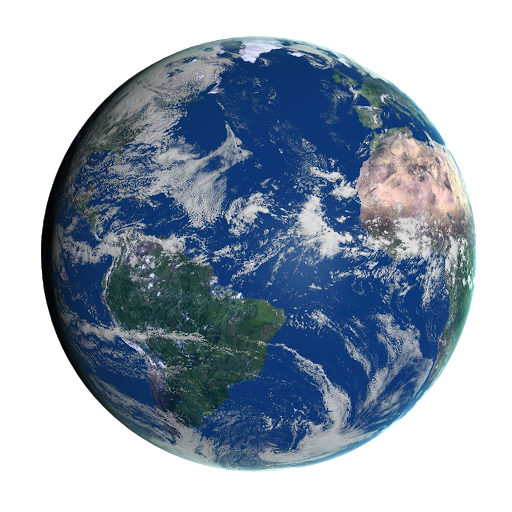
\includegraphics[width=0.2\textwidth]{figs/reality.png}
	\end{figure}

%\pause

\begin{center}
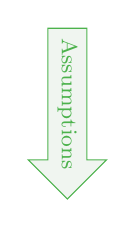
\begin{tikzpicture}[every node/.style={single arrow, draw=none, rotate=-90}]
\node [draw=green!40!gray,fill=green!20!gray!10,text=green!40!gray,font=\footnotesize] {Assumptions};
\end{tikzpicture}
\end{center}


\usetikzlibrary{shapes,arrows}
\tikzstyle{block} = [draw, rectangle, minimum height=3em, minimum width=6em]
\tikzstyle{input} = [coordinate]
\tikzstyle{output} = [coordinate]

\begin{figure}
\centering 
\begin{tikzpicture}[auto, node distance=4cm, >=latex, very thick]
    \node [input, name=input] {};
    \node [block, right of=input, text width=2cm] (system) {\begin{center} SYSTEM\\\medskip production \end{center} };
    \node [output, right of=system] (output) {};
    \draw [->] (input) -- node[above] {incoming} (system) {};
    \draw [->] (system) -- node[above] {outgoing} (output) {};
\end{tikzpicture}
\end{figure}
	
%\pause	
	\color{ugent-la}
	\begin{equation*} 
		\left[
		\frac{accumulation}{time}
		\right]=
		\left[
		\frac{production}{time}
		\right]
		+
		\underbrace{
			\left[
			\frac{incoming}{time}
			\right]-\left[
			\frac{outgoing}{time}
			\right]}_{transport}
		\label{eq:massconsdyn}
		\end{equation*}
	
}

\frame{
	
	\begin{figure}
		\begin{minipage}[b]{0.23\linewidth}
			\centering
			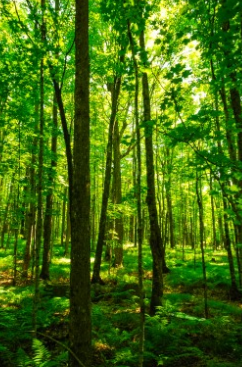
\includegraphics[height=2.5cm]{figs/bos}
			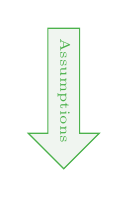
\begin{tikzpicture}[every node/.style={single arrow, draw=none, rotate=-90}]
			\node [draw=green!40!gray,fill=green!20!gray!10,text=green!40!gray,font=\tiny] {Assumptions};
			\end{tikzpicture}
			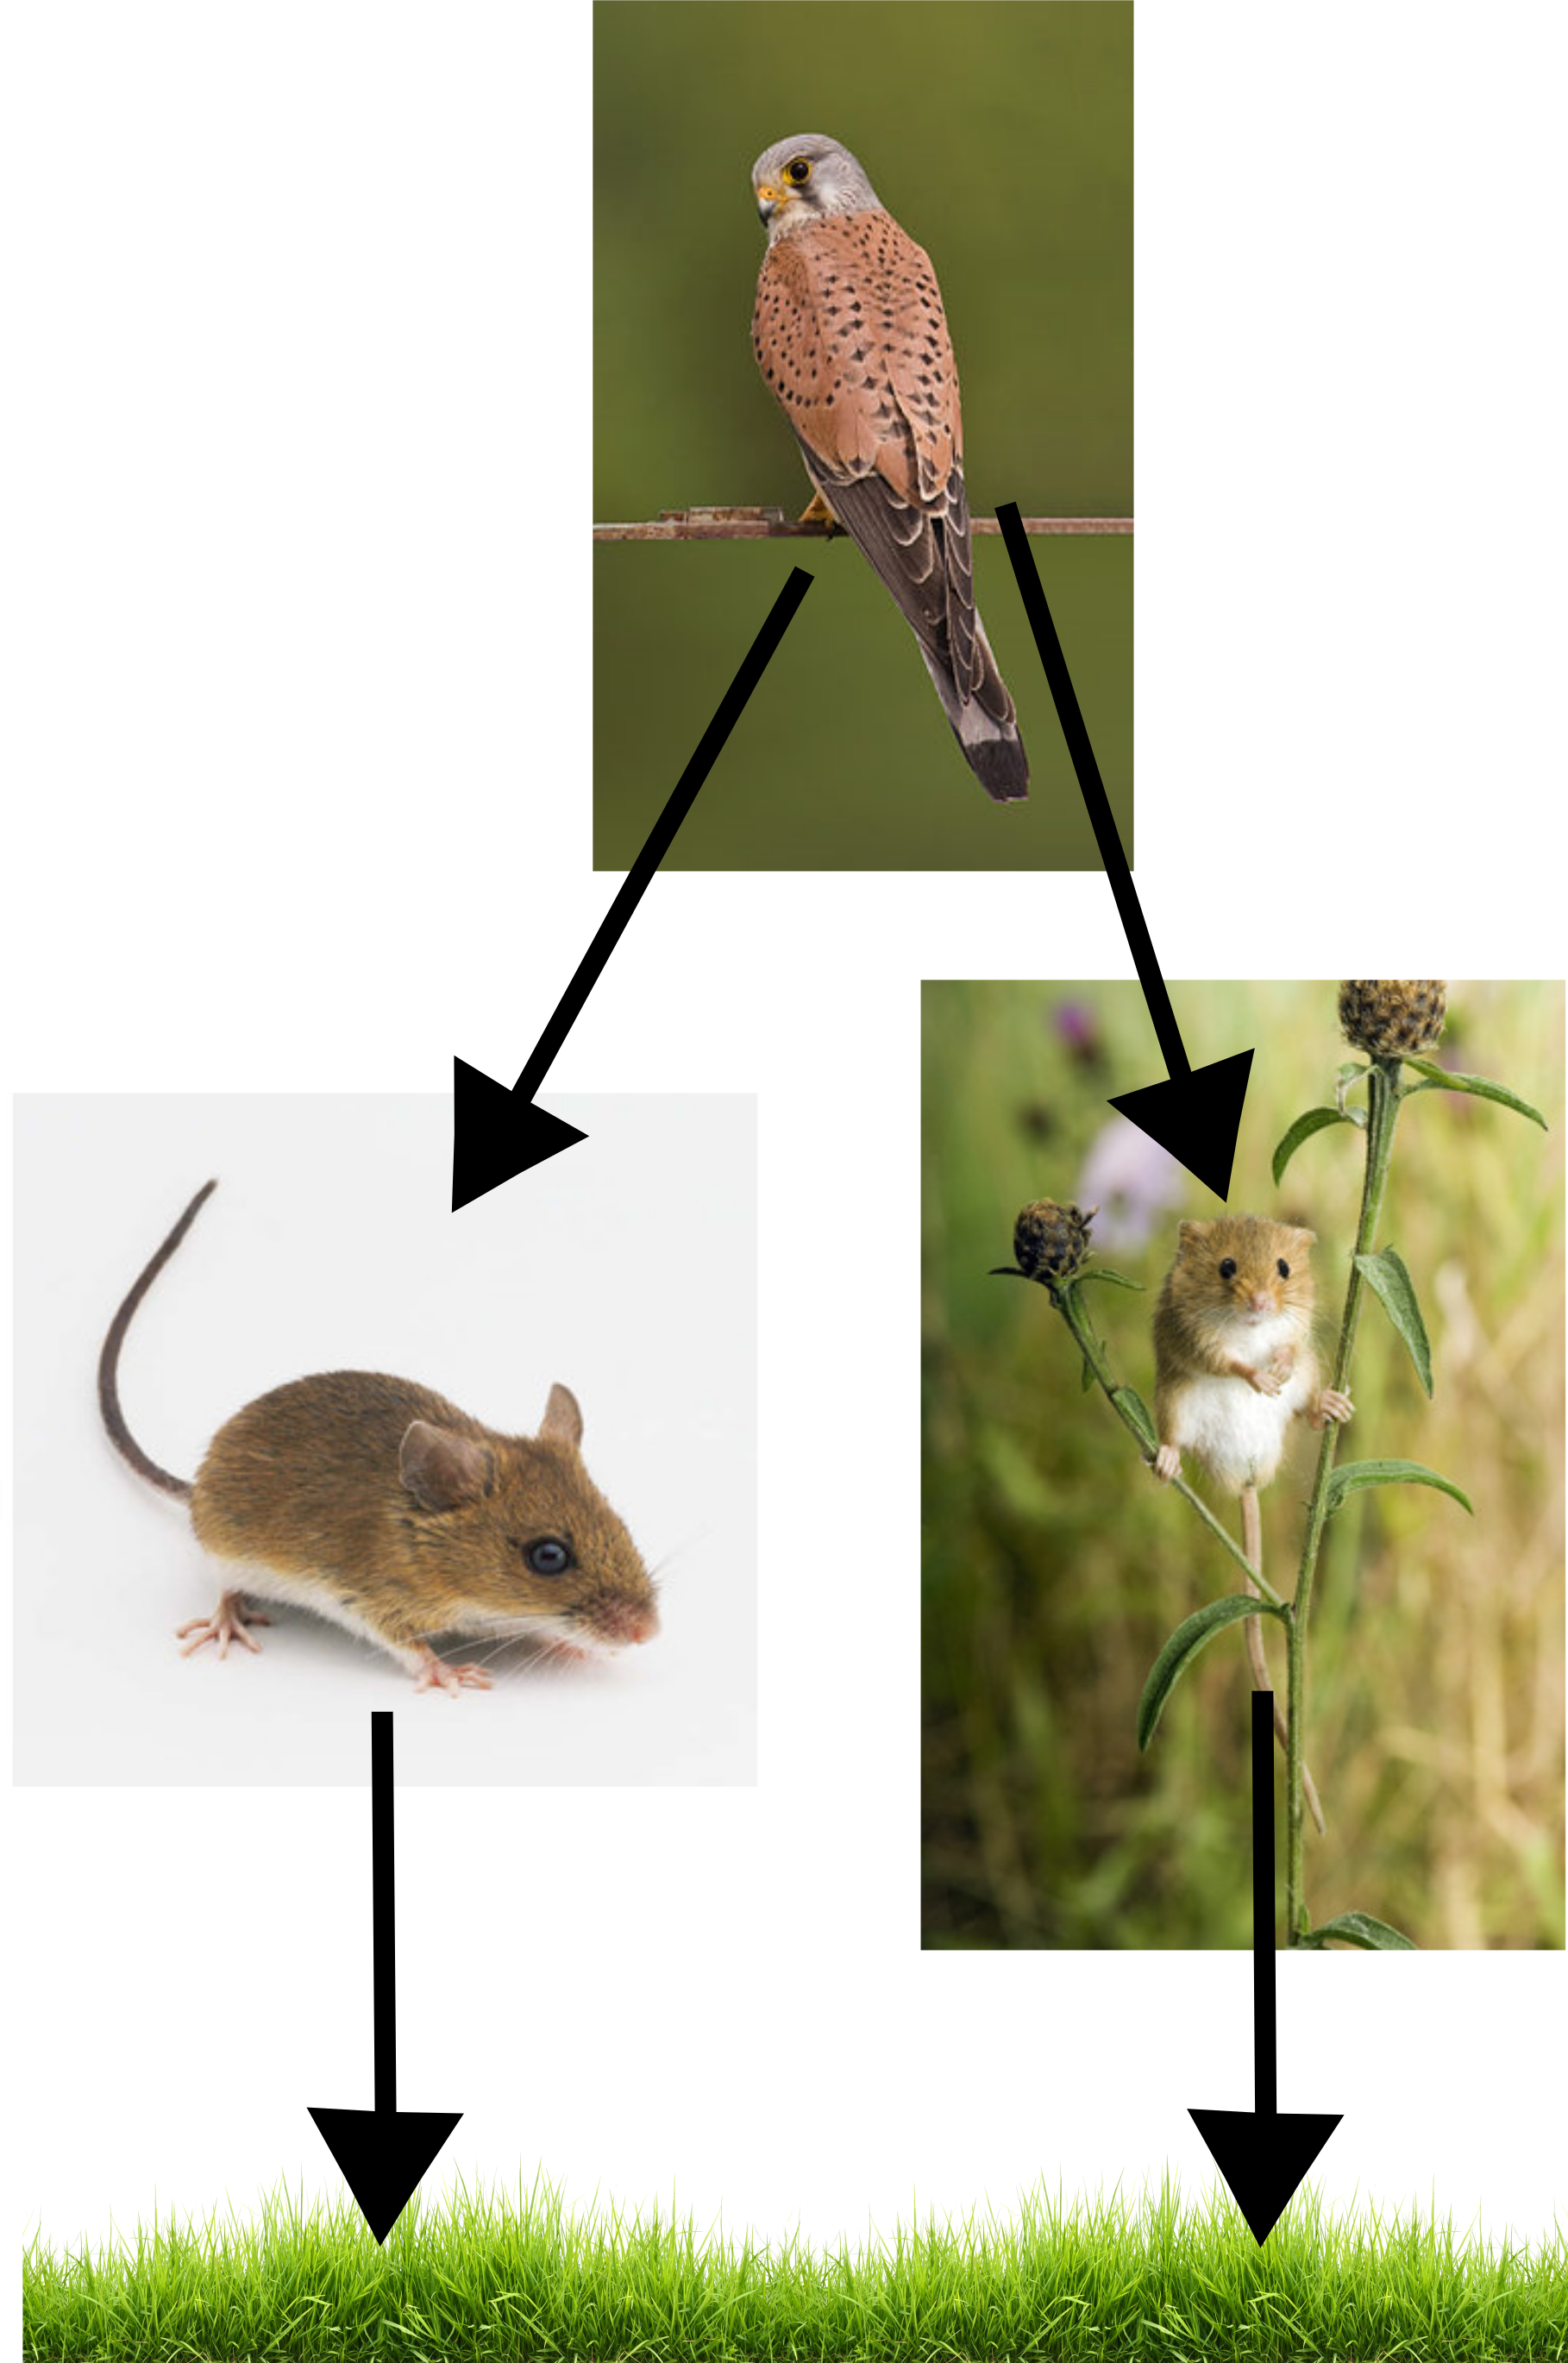
\includegraphics[height=2.5cm]{figs/foodweb}
			\color{ugent-la}{\begin{equation*} 
					\frac{d v}{d t}
				\end{equation*}}
		\end{minipage}
		\hspace{0.05cm}
		\begin{minipage}[b]{0.23\linewidth}
			\centering
			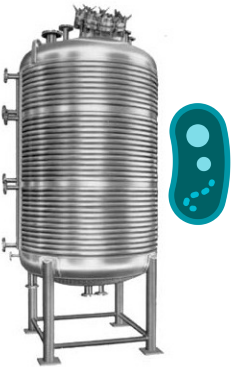
\includegraphics[height=2.5cm]{figs/reactorBio}
			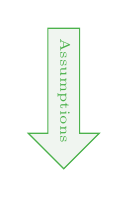
\begin{tikzpicture}[every node/.style={single arrow, draw=none, rotate=-90}]
			\node [draw=green!40!gray,fill=green!20!gray!10,text=green!40!gray,font=\tiny] {Assumptions};
			\end{tikzpicture}
			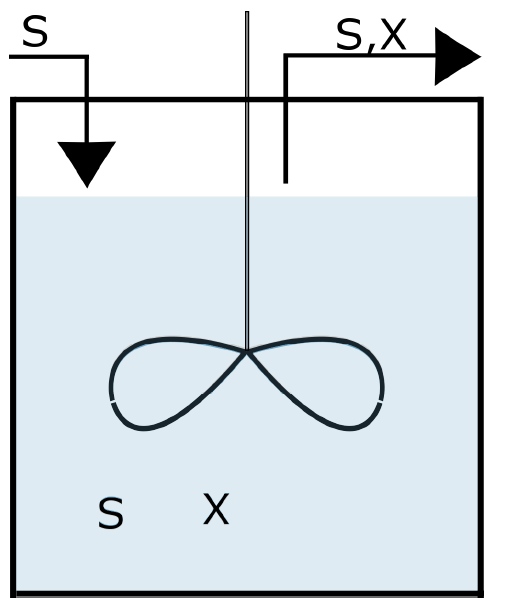
\includegraphics[height=2.5cm]{figs/reactorBioM}
			\color{ugent-la}{\begin{equation*} 
				\frac{d[X]}{d t}
				\end{equation*}}
		\end{minipage}
		\hspace{0.05cm}
		\begin{minipage}[b]{0.23\linewidth}
			\centering
			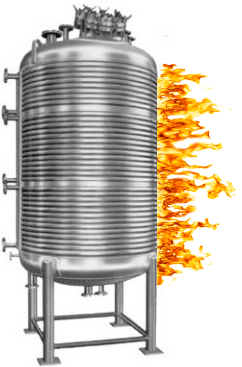
\includegraphics[height=2.5cm]{figs/reactorVuur}
			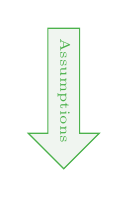
\begin{tikzpicture}[every node/.style={single arrow, draw=none, rotate=-90}]
			\node [draw=green!40!gray,fill=green!20!gray!10,text=green!40!gray,font=\tiny] {Assumptions};
			\end{tikzpicture}
			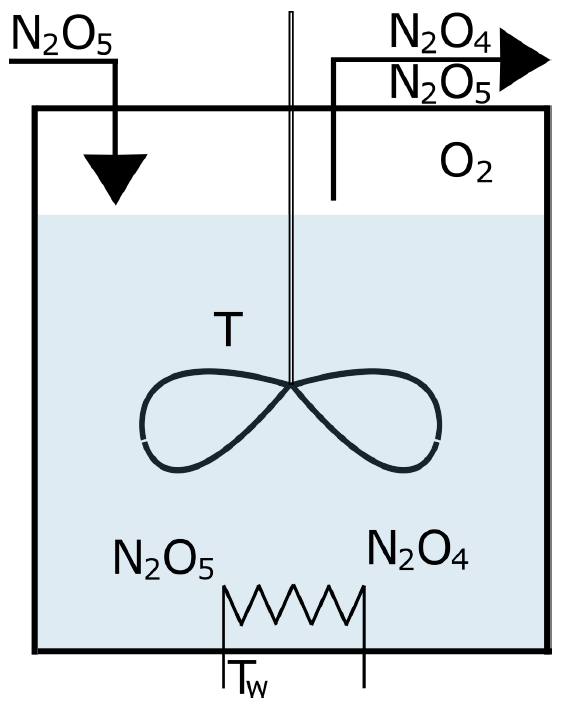
\includegraphics[height=2.5cm]{figs/reactorVuurM}
			\color{ugent-la}{\begin{equation*} 
				\frac{d T}{d t}
				\end{equation*}}
		\end{minipage}
		\hspace{0.05cm}
		\begin{minipage}[b]{0.23\linewidth}
			\centering
			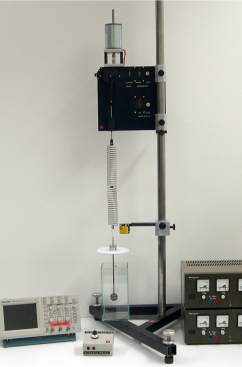
\includegraphics[height=2.5cm]{figs/osc}
			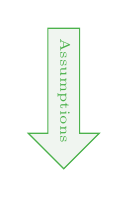
\begin{tikzpicture}[every node/.style={single arrow, draw=none, rotate=-90}]
			\node [draw=green!40!gray,fill=green!20!gray!10,text=green!40!gray,font=\tiny] {Assumptions};
			\end{tikzpicture}
			
			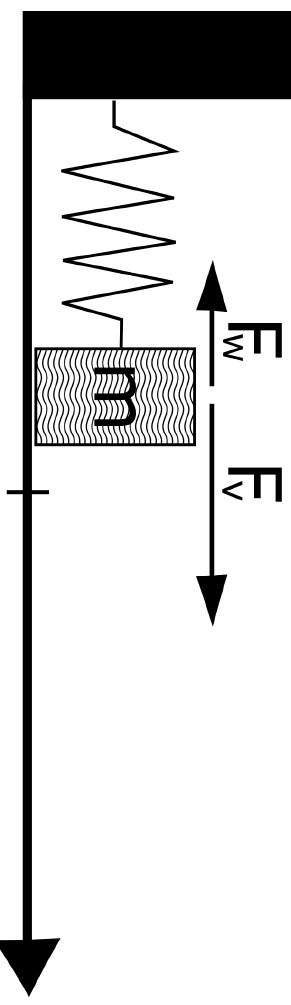
\includegraphics[height=2.5cm]{figs/oscM}
			\color{ugent-la}{\begin{equation*} 
				\frac{d^2 x}{d t^2}
				\end{equation*}}
		\end{minipage}
	\end{figure}
	
}

\frame{
  \frametitle{Goal of this practicum}
  \Large
  \color{beamerstructure}
  {\begin{enumerate}
	\item Implementing \textit{reaction systems} using Catalyst
	\vfill %\pause
	\item Understanding the relation with balance equations
	\vfill %\pause
	\item Simulation of systems as ODE-problems
	\vfill %\pause
	\item Influence of parameters
	\vfill %\pause
	\item Implementing \textbf{discrete events}
	\vfill %\pause
	\item Implementing \textbf{continuous events}
  \end{enumerate}
  }
}

\frame{
\frametitle{Introduction to Catalyst}
\Large
\begin{itemize}
\item Symbolic modelling package for construction, analysis and high performance simulation of chemical reaction networks.
\vfill
\item Catalyst defines symbolic ReactionSystems, created using Catalyst's \textbf{D}omain \textbf{S}pecific \textbf{L}anguage (DSL).
\vfill
\end{itemize}
}

\frame{
\frametitle{Introduction to Catalyst}
\Large

The infection model \bigskip

\begin{figure}
	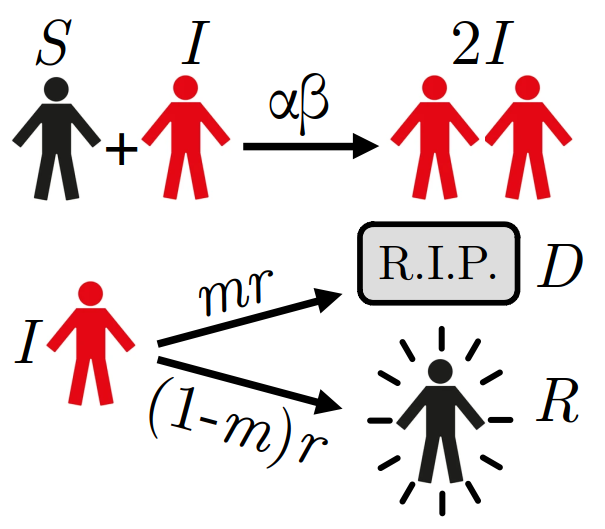
\includegraphics[width=0.6\textwidth]{figs/infection_model.png}
\end{figure}
}


\frame{
\frametitle{Introduction to Catalyst}
\Large

The infection model - \textit{reaction network system}

$$S + I \xrightarrow[]{\alpha \beta} 2I$$
$$I \xrightarrow[]{mr} D$$
$$I \xrightarrow[]{(1-m)r} R$$

Implementation

\begin{figure}
	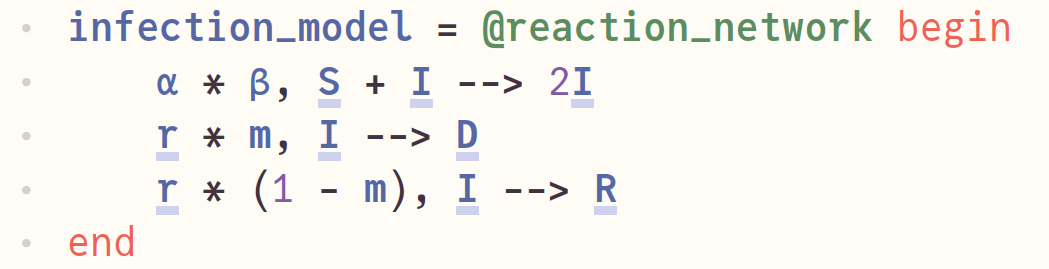
\includegraphics[width=0.7\textwidth]{figs/infection_model_catalyst_implementation.png}
\end{figure}

$S$, $I$, $D$ and $R$ are called species, unknowns or states\\
$\alpha$, $\beta$, $m$, $r$ are called parameters
}


\frame{
\frametitle{Introduction to Catalyst}
\Large

The infection model - corresponding \textit{system of ODEs}

\begin{eqnarray*}
\cfrac{dS}{dt} &=& -\alpha \beta S I \\
\cfrac{dI}{dt} &=& \alpha \beta S I - r I \\
\cfrac{dD}{dt} &=& m r I \\
\cfrac{dR}{dt} &=& (1-m) r I
\end{eqnarray*}

}


\frame{
\frametitle{Introduction to Catalyst}
\Large
For a given problem it is: \medskip
\begin{itemize}
\item Sometimes easier to immediately write down the \textbf{reaction network} (reaction kinetics), e.g., for chemistry, biological, population and epidemiological related problems. \medskip
\item Sometimes easier to write down the \textbf{system of ODEs}, e.g., for environmental and physics related problems. In the latter case you will need to ``translate'' it into a reaction network.
\end{itemize}
}


%\frame{
%\frametitle{Pluto notebooks}
%\large \bigskip
%All exercises will be in the form of Pluto notebooks. You will find them on Ufora in a submodule of the module \textbf{Exercises}. \medskip
%\begin{itemize}
%\item For this practicum, go to the Ufora submodule\\ \textbf{P1: ODEs 1 $>$ files} \medskip
%\item Download the Julia script \texttt{launch\_pluto.jl} and all the Pluto notebooks (\texttt{e.g., ode\_model\_catalyst\_intro.jl}, etc.) into your dedicated \texttt{modsim} folder. \medskip
%\begin{itemize} 
%\item \texttt{launch\_pluto.jl} is a small script to activate your environment and to be able to use the packages you installed in your environment. \medskip
%\end{itemize}
%\item Go to your dedicated folder (cf. \texttt{modsim}) with a \textit{File Explorer}, then in this location right click on your mouse and choose \texttt{Open in Terminal} (or something alike). \medskip
%\item Type {\color{ugent-la} \texttt{julia launch\_pluto.jl}} and then click [\textit{Enter}] \medskip
%\item The Pluto notebook of you choice will open in your browser.
%\end{itemize}
%}


\frame{
\frametitle{Practicum 1: ODEs 1}
\large
The following notebooks are the subjects for today:
\begin{itemize}
\item \texttt{ode\_model\_catalyst\_intro.jl} (introduction) \vspace*{2mm}
\item \texttt{ode\_model\_infection.jl}
\item \texttt{ode\_model\_birth\_death.jl}
\item \texttt{ode\_model\_irrigation.jl} \vspace*{2mm}
\item \texttt{ode\_model\_fermenter\_firstorder.jl} (extra)
\item \texttt{ode\_model\_fermenter\_monod.jl} (extra)
\item \texttt{ode\_model\_soil\_cont\_plant\_uptake.jl} (extra)
\item \texttt{ode\_model\_water\_evap\_infil.jl} (extra)
\item \texttt{ode\_model\_anaerobic\_fermentation.jl} (extra)
\end{itemize}
}



\frame{
\frametitle{Intro to Catalyst - ODEs}
\large
We will use the infection model to illustrate the following: \medskip
\begin{itemize}
\item Implementation of the system as a \textit{reaction network} object using Catalyst's DSL \medskip
\item Simulation of the system as an ODE-problem \medskip
\item Some advanced examples:
\begin{itemize}
\item How to analyse the \textit{influence of a parameter} \smallskip
\item Introduce a \textit{discrete event} in time \smallskip
\item Introduce a \textit{continuous event}
\end{itemize}
\end{itemize}
}


\frame{
\frametitle{Intro to Catalyst - ODEs}
\Large \bigskip

Notebook: {\color{ugent-la} \texttt{ode\_model\_catalyst\_intro.jl}}

\medskip
The infection model: \medskip

\begin{figure}
	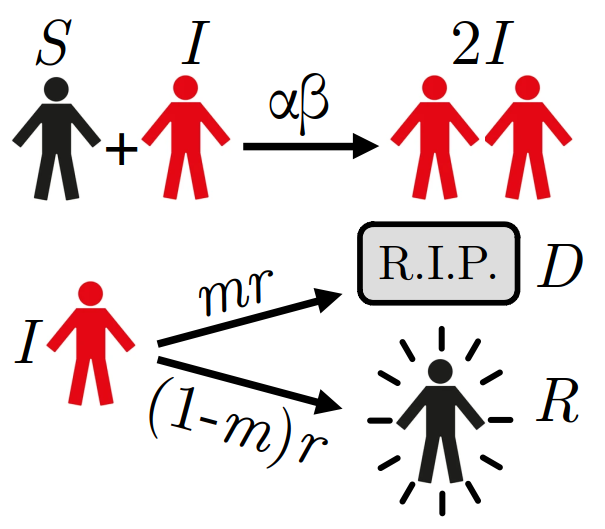
\includegraphics[width=0.6\textwidth]{figs/infection_model.png}
\end{figure}
}

\frame{
\frametitle{Exercise 1}
\Large
\textbf{The infection model}\\ \medskip
Notebook: {\color{ugent-la}\texttt{ode\_model\_infection.jl}}

\begin{itemize}
\item Contains the code from the introduction notebook (minimal explanatory text) \medskip
\item Influence of parameter $\alpha$ \medskip
\item Administration of medicinal products \medskip
\item Adding vaccination to the model
\end{itemize}
}


\frame{
\frametitle{Exercise 2}
\Large
\textbf{Simple birth-death model for mice}\\ \medskip
Notebook: {\color{ugent-la}\texttt{ode\_model\_birth\_death.jl}}

\vspace*{2mm}
Part 1

\begin{figure}
	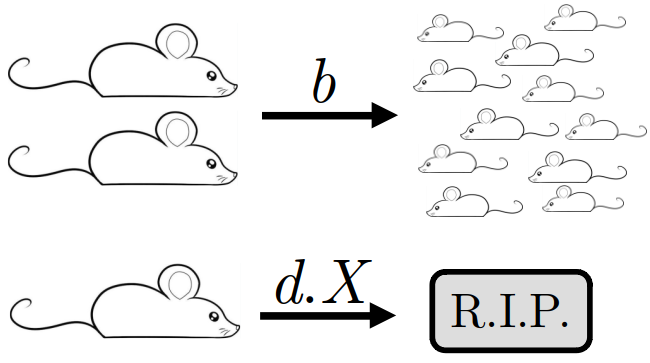
\includegraphics[width=0.8\textwidth]{figs/mice_model_part1.png}
\end{figure}
}


\frame{
\frametitle{Exercise 2}
\Large \medskip
\textbf{Simple birth-death model for mice}\\ \medskip
Notebook: {\color{ugent-la}\texttt{ode\_model\_birth\_death.jl}}

\vspace*{2mm}
Part 2

\begin{figure}
	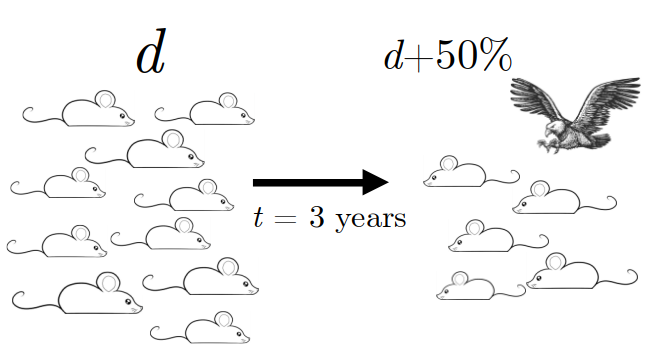
\includegraphics[width=0.8\textwidth]{figs/mice_model_part2.png}
\end{figure}
}


\frame{
\frametitle{Exercise 3}
\Large
\textbf{Irrigation experiment}\\ \medskip
Notebook: {\color{ugent-la}\texttt{ode\_model\_irrigation.jl}}

\begin{figure}
	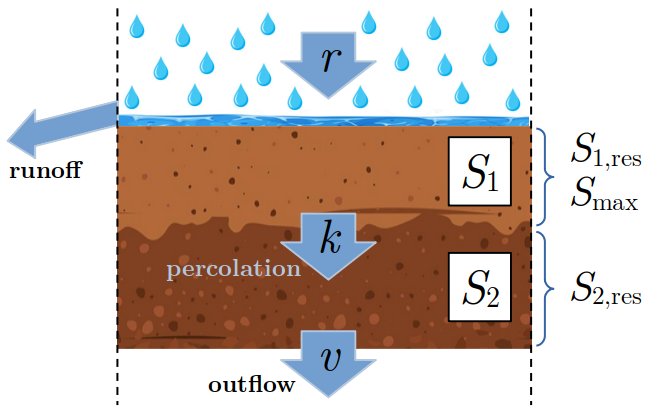
\includegraphics[width=0.8\textwidth]{figs/irrigation_model.png}
\end{figure}
}


\frame{
\frametitle{Extra exercises 4 and 5}
\Large
\textbf{Fermenter}\\ \medskip
Notebooks: {\color{ugent-la}\texttt{ode\_model\_fermenter\_firstorder.jl}} and {\color{ugent-la}\texttt{ode\_model\_fermenter\_monod.jl}}

\begin{figure}
	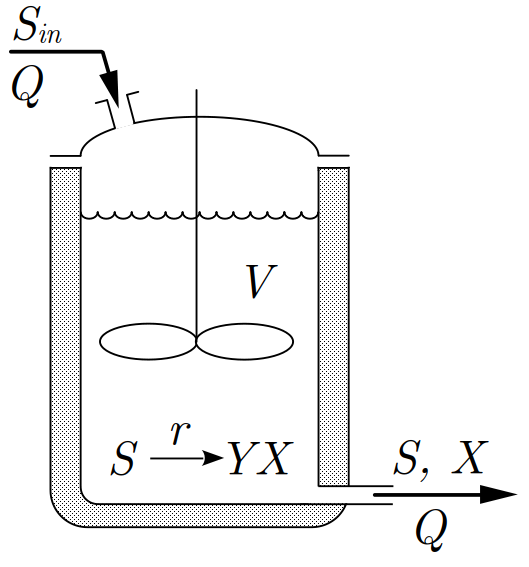
\includegraphics[width=0.5\textwidth]{figs/fermenter_model.png}
\end{figure}
}


\frame{
\frametitle{Extra exercise 6}
\Large \medskip
\textbf{Soil contamination with plant uptake}\\ \medskip
Notebook: {\color{ugent-la}\texttt{ode\_model\_soil\_cont\_plant\_uptake.jl}}

\begin{figure}
	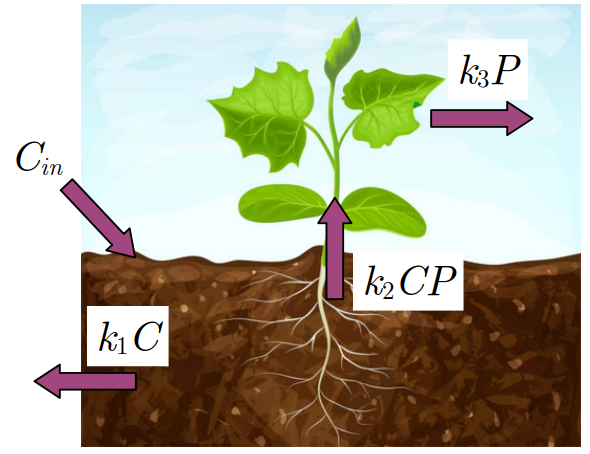
\includegraphics[width=0.7\textwidth]{figs/soil_plant_cont_model.png}
\end{figure}
}


\frame{
\frametitle{Extra exercise 7}
\Large \medskip
\textbf{Water evaporation and infiltration}\\ \medskip
Notebook: {\color{ugent-la}\texttt{ode\_model\_water\_evap\_infil.jl}}

\begin{figure}
	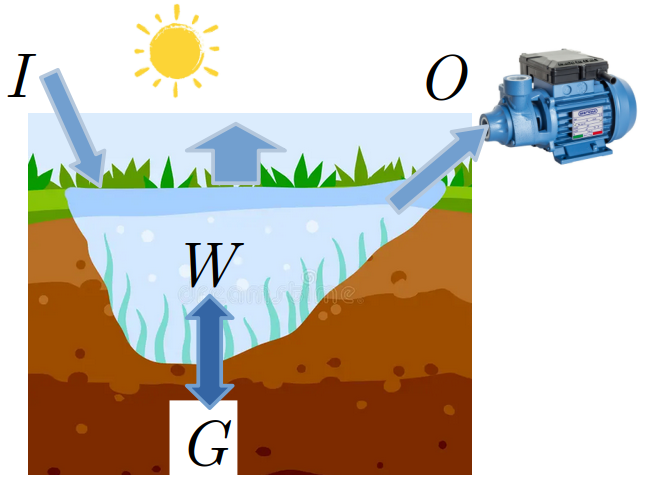
\includegraphics[width=0.7\textwidth]{figs/water_evap_infil_model.png}
\end{figure}
}

\frame{
\frametitle{Extra exercise 8}
\Large
\textbf{Anaerobic fermentation}\\ \medskip
Notebook: {\color{ugent-la}\texttt{ode\_model\_anaerobic\_fermentation.jl}}

\begin{figure}
	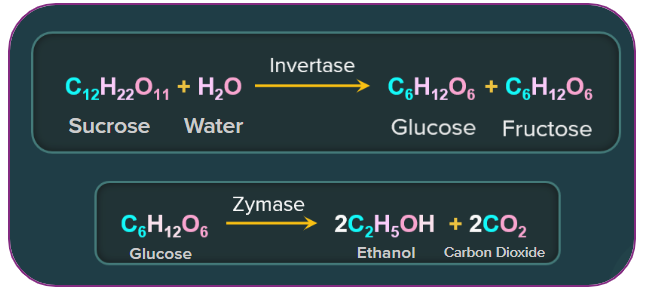
\includegraphics[width=0.7\textwidth]{figs/anaerobic_fermentation.png}
\end{figure}
}


\end{document}

